

\chapter{基于输入图片多尺寸放大的卷积神经网络显著图解释方法}
\thispagestyle{others}
\pagestyle{others}
\xiaosi

\section{本章引言}



\section{问题描述和研究思路}
当前大多数基于类激活映射的显著图解释方法诸如CAM、Grad-CAM、Grad-CAM++、XGrad-CAM、Score-CAM等都存在一个共有问题,即最终生成的显著图的分辨率较低,这导致其只能在显著图中呈现一个模糊的解释效果,无法聚焦更加精细的特征。究其原因是这些基于类激活映射的方法一般提取的都是卷积神经网络的最后一层卷积层的输出作为特征图的来源,因该层包含较为丰富的类别特征信息,之后通过各种加权方法组合这些特征图来得到最终的显著图。因为卷积神经网络的结构特性,其最后一层卷积层的会输出多个通道的低分辨率特征图,因此无论如何组合这些特征图,最终得到的也只是一张分辨率和最后一层的卷积层输出的单一通道的特征图相当的初级显著图。当然一般情况下为了得到显著图和原始输入图片的特征对应关系,都会将这张原始输入图片进行分辨率层面的放大,使用的一般也是双线性插值算法,但这并不意味着原始显著图的有效信息的增多。

这里以VGG19这个基于卷积神经网络的图片分类模型举例,若输入图片的尺寸是3$\times$224$\times$224,其中3表示RGB颜色通道,224$\times$224表示图片分辨率,那么该模型最后一层卷积层的输出的特征图尺寸是512$\times$14$\times$14,其中数字512是通道数量,14$\times$14是特征图的分辨率。若我们使用双线性插值函数$\phi(s,H,W)$将原始显著图分辨率提升到224$\times$224,那么意味着我们插入了额外99.9\%的信息,而最终的显著图中的这些额外的像素信息并不能反映图片分类模型对原始输入图片的对应像素的感兴趣程度。即便有部分文献\textsuperscript{\cite{adebayo2018sanity}\cite{selvaraju2017grad}}试图改进这种插值函数,但是它们仍然引入了外部不相关的信息。

因此为了解决上述的问题,本文从特征图的提取这一关键点着手。考虑到若使用原始输入图片,那么卷积神经网络最后一层卷积层输出的单一特征图分辨率较低且包含的特征信息有限,因此本文提出基于输入图片多尺寸放大的卷积神经网络显著图解释方法,其核心就是将输入图片进行逐级多尺寸的双线性插值放大,例如将输入图片放大至334$\times$334、434$\times$434、534$\times$534等分辨率,这时能得到一组分辨率不同的输入图片,接着将这组输入图片分别送入基于卷积神经网络的图像分类模型中,再从其最后一层卷积层中分别提取特征图和梯度矩阵数据,基于卷积神经网络的采样特性,可以得到不同分辨率的特征图,更高分辨率的输入图片即对应更高分辨率的特征图,也即拥有更丰富的特征信息。因此若将这些特征图的信息进行融合即能得到分辨率更高的掩膜,再用这些更高分辨率的掩膜对原始输入图片进行扰动,即可得到相应的掩膜权重,用权重和高分辨率掩膜进行融合即能得到包含更多特征信息并且分辨率更高的显著图。
\section{基于输入图片多尺寸放大的卷积神经网络显著图解释方法}


\subsection{生成高分辨率掩膜}
令原始输入图片为$I_0 \in \mathbb{R}^{3\times H_0 \times W_0}$,其中3表示RGB颜色通道数量,$H_0$和$W_0$分别原始输入图片的长和宽的像素个数,即原始输入图片的分辨率可以表示为$\zeta_0=(H_0,W_0)$。此外,我们用$\mathcal{F}$表示一个预训练好的基于卷积神经网络的图像分类模型,那么$\mathcal{F}_c(I_0)$则表示在输入图片为$I_0$的情况下,图像分类模型$\mathcal{F}$对于类别$c$的输出分数,值得注意的是,该分数是未经归一化指数函数(softmax函数)之前的分数。将原始输入图片送入图像分类模型$\mathcal{F}$,并从其最后一层卷积层$l$当中提取所有通道的特征图集合,该特征图集合表示为$\overset{*}{\boldsymbol{A}_0}$。通过获得的类别$c$的输出分数$\mathcal{F}_c(I_0)$,对该分数反向传播至最后一层卷积层特征图,则可以获得对应特征图关于类别$c$的梯度矩阵$\overset{*}{\boldsymbol{G}_0}$,计算公式如下:
\begin{equation}
\overset{*}{\boldsymbol{G}_0}=\frac{\partial \mathcal{F}_c(I_0)}{\partial \overset{*}{\boldsymbol{A}_0}}
\label{eq:g0}
\end{equation}
\ref{eq:g0}公式中,梯度矩阵集合$\overset{*}{\boldsymbol{G}_0}$一共有$K$个通道,通道数量和特征图集合$\overset{*}{\boldsymbol{A}_0}$一致,并且每个通道的梯度矩阵和特征图一一对应。 

接着将原始输入图片$I_0$经由双线性插值函数$\varphi(I_0,\zeta_t)$上采样至图片$I_t$,$t$表示第$t$次上采样结果,经由上采样后的$I_t$的分辨率可表示为$\zeta_t$,$\zeta_t$是由于原始输入图片的分辨率$\zeta_0$逐步递增得来的。为了控制计算的时间成本,考虑将$\zeta_{max}=(H_{max},W_{max})$作为上采样分辨率的上限,同时设$N$为最大迭代次数即上采样次数,那么第$t$次上采样得到的图片分辨率可由以下公式计算得出:
\begin{equation}
	\zeta_t=\zeta_0 +\lfloor\frac{\zeta_{max}}{N}\rfloor(t-1)
\end{equation}
在上述迭代过程当中,每次上采样获得的输入图片$I_t$的分辨率都不同,则将其输入到图像分类模型当中$\mathcal{F}$从最后一层卷积层提取的特征图集合$\overset{*}{\boldsymbol{A}_t}$的分辨率也不同,而且随着输入图片分辨率的提高,$\overset{*}{\boldsymbol{A}_t}$的分辨率也会相应提高,相对应的$\overset{*}{\boldsymbol{A}_t}$也能包含更多和类别$c$相关的细节特征信息。因此若将这些不同的分辨率的特征图集合进行融合则能够得到更多的特征信息。融合的方法可由以下的公式进行表示:
\begin{equation}
	\overline{\bm{A}}=\frac{1}{t_{max}}\sum_{t=0}^{t_{max}}\varphi(\overset{*}{\boldsymbol{A}_t},\zeta_0)
	\label{eq:Afuse}
\end{equation}
公式\ref{eq:Afuse}中,$t_{max}$表示最大的有效迭代次数,此处的“有效”指的是只有当图像分类模型的输出结果中概率分数最大的类别是$c$时才采用这次迭代的特征图集合$\overset{*}{\boldsymbol{A}_t}$,其他情况下均舍弃,因此不难得出$t_{max} \leq N$。同时$\varphi(\overset{*}{\boldsymbol{A}_t},\zeta_0)$表示将特征图集合$\overset{*}{\boldsymbol{A}_t}$中的每一个通道上的特征图均上采样至原始输入图片的分辨率$\zeta_0$,这样做的目的是方便将不同分辨率的特征图集合进行融合,也方便后续对原始输入图片进行扰动。

在每次迭代过程中,都会计算并提取保存图像分类模型关于类别c的输出分数$\mathcal{F}_c(I_t)$对于卷积层$l$的特征图集合$\overset{*}{\boldsymbol{A}_t}$的反向传播梯度$\overset{*}{\boldsymbol{G}_t}$,和特征图集合一样,将不同迭代过程中保存的梯度矩阵集合$\overset{*}{\boldsymbol{G}_t}$也进行融合,可以得到$\overline{\bm{A}}$分辨率尺寸一致梯度矩阵集合,融合的公式如下所示:
\begin{equation}
	\overline{\bm{G}}=\frac{1}{t_{max}}\sum_{t=0}^{t_{max}}\varphi(\overset{*}{\boldsymbol{G}_t},\zeta_0)
	\label{eq:Gfuse}
\end{equation}
同样,公式\ref{eq:Gfuse}中,同时$\varphi(\overset{*}{\boldsymbol{G}_t},\zeta_0)$表示将梯度矩阵集合$\overset{*}{\boldsymbol{G}_t}$中的每一个通道上的梯度矩阵均上采样至原始输入图片的分辨率$\zeta_0$。由于融合后的特征图集合中不仅包含类别$c$特征信息,也包含其他类别的特征信息,因此为了将类别$c$的特征信息进行凸显,其他类别的特征信息进行削弱,我们将利用融合后的梯度矩阵$\overline{\bm{G}}$,它在一定程度上反映了特征图上不同像素对类别分数$\mathcal{F}_c(I_0)$的敏感程度,或者说是重要程度\textsuperscript{\cite{selvaraju2017grad}3}。仿照Grad-CAM\textsuperscript{\cite{selvaraju2017grad}4}中的方法,我们将$\overline{\bm{G}}$中每张梯度矩阵进行全局平均池化,在每个通道上得到一个权重值,每个通道下的权重值都和$\overline{\bm{A}}$中的每个通道下的特征图一一对应,所有通道下权重值的集合的计算公式如下:
\begin{equation}
	\overline{\bm{W}}=\frac{1}{H_0\times W_0}\sum_{i=1}^{H_0}\sum_{j=1}^{W_0}\overline{\bm{G}}
	\label{eq:Wfuse}
\end{equation}
额外说明的是,融合后的特征图集合$\overline{\bm{A}}$的尺寸是$[1\times K \times H_0\times W_0]$,它对应的权重集合$\overline{\bm{W}}$的尺寸是$[1\times K \times 1\times 1]$,其中$K$就是第$l$层卷积层输出的特征图通道数量。

本小节的最后,初始掩膜集合$\boldsymbol{M}$可以通过以下公式计算得出:
\begin{equation}
	\boldsymbol{M}=	\overline{\bm{A}}\cdot\overline{\bm{W}}
\end{equation}
其中,运算符$\cdot$表示$\overline{\bm{A}}$中的每个通道下的特征图中的每个像素值都和$\overline{\boldsymbol{W}}$中对应每个权值相乘。

\subsection{掩膜优化}
$\boldsymbol{M}$是经由输入图片多尺寸上采样放大后从卷积层中提取的特征图和梯度矩阵结合而得到的,相比单一原始输入图片得到掩膜(比如Score-CAM\textsuperscript{\cite{wang2020score}2}),$\boldsymbol{M}$包含更丰富的类别特征信息,但是目前得到$\boldsymbol{M}$仍然不能直接当作掩膜来扰动输入图片,它还有两个明显的缺点。第一点是$\boldsymbol{M}$的尺寸是$[1\times K \times H_0\times W_0]$,其中$K$是卷积层$l$输出的特征图的通道数量,一般我们取最后一层卷积层作为$l$,因此$K$的值将会是数百至上千,显然这样掩膜的数量太多了,若像Score-CAM\textsuperscript{\cite{wang2020score}3}一样逐个将掩膜去扰动原始输入图片得到权值,那样将会极为耗时。第二个缺点$\boldsymbol{M}$就是使用全局平均池化后的梯度作为特征图的权重,由于ReLU函数的零梯度问题\textsuperscript{\cite{zhang2021novel}},这意味着$\boldsymbol{M}$显然会有噪声。因此,为了使$\boldsymbol{M}$成为合格的掩膜,需要让它变得更加纯净。

\begin{algorithm}
	\caption{MSG-CAM}
	\label{alg:1}
	\renewcommand{\algorithmicrequire}{\textbf{输入:}}
	\renewcommand{\algorithmicensure}{\textbf{输出:}}
	\begin{algorithmic}[1]
		\REQUIRE 基于卷积神经网络的图像分类模型 $\mathcal{F} $ ,原始输入图片 $I_0 \in \mathbb{R}^{3\times H_0 \times W_0}$ ,上采样分辨率上限 $\zeta_{max}=(H_{max},W_{max})$ ,卷积层 $l$ ,最大迭代次数 $N$ ,类别 $c$ ,每个分组中掩膜数量$B$, 高斯模糊参数: $kernel\_size,sigma$, interpolation function $\varphi(.)$
		\ENSURE 显著图 $L_{MSG-CAM}\in \mathbb{R}^{3\times H_0 \times W_0}$
		\STATE 初始化 $L_{MSG-CAM} \leftarrow 0$ , $\mathcal{A}_0 \leftarrow 0$ , $\mathcal{G}_0 \leftarrow 0$ , $r \leftarrow 0$ , $t_{max}\leftarrow 0$ , $t_m\leftarrow 0$ , $kernel\_size=51,sigma=50$ ,基准图片 $I^{\prime}_0=guassian\_blur2d(I_0,kernel\_size,sigma)$ , $c=\mathcal{F}(I_0)$
		\WHILE{$t\leq N$}
		\STATE $t\leftarrow t+1$
		\STATE $\zeta_t\leftarrow \zeta_0 +\lfloor\frac{\zeta_{max}}{N}\rfloor(t-1)$
		\STATE $I_t\leftarrow \varphi(I_0,\zeta_t)$
		\IF{$\mathcal{F}(I_t) \rightarrow c$}
		\STATE $t_{max}\leftarrow t_{max}+1$
		\STATE $\overset{*}{\boldsymbol{A}_t}\leftarrow \mathcal{A}(I_t,l)$
		\STATE $\overset{*}{\boldsymbol{G}_t}\leftarrow \nabla\mathcal{J}(l,c)$
		\STATE $\mathcal{A}_t \leftarrow \mathcal{A}_{t-1}+\varphi(\overset{*}{\boldsymbol{A}_t},\zeta_0)$
		\STATE $\mathcal{G}_t \leftarrow \mathcal{G}_{t-1}+\varphi(\overset{*}{\boldsymbol{G}_t},\zeta_0)$
		\ENDIF
		\ENDWHILE
		\STATE $\overline{\bm{A}}\leftarrow \mathcal{A}_t/t_{max}$
		\STATE $\overline{\bm{G}}\leftarrow \mathcal{G}_t/t_{max}$
		\STATE $\overline{\bm{W}}\leftarrow \frac{1}{m\times n}\sum_{i=i}^{m}\sum_{j=1}^{n}\overline{\bm{G}}$
		\STATE $\boldsymbol{M}=\overline{\bm{A}}\cdot\overline{\bm{W}}$
		\STATE $K\leftarrow$ $\boldsymbol{M}$的通道数量;
		\STATE $g\leftarrow$ 每个分组中掩膜数量;
		\WHILE{$r<B$}
		\STATE 在组内生成单一的掩膜\\ $M_r=ReLU(\sum_{k=r\times g}^{(r+1)\times g-1}M^k)$
		\STATE 初始化 $M^{\prime}_r\leftarrow$ 将$M^r$进行去噪操作和归一化
		\STATE 用掩膜扰动原始输入图片\\$I_r=I_0\odot M^{\prime}_r+I^{\prime}_0\odot (1-M^{\prime}_r)$
		\STATE 计算每张掩膜的权重\\$\alpha_r=\mathcal{F}_c(I_r)-\mathcal{F}_c(I^{\prime}_0)$
		\STATE $L_{MSG-CAM}\leftarrow L_{MSG-CAM}+\alpha_r M_r$
		\STATE $r\leftarrow r+1$
		\ENDWHILE
		\RETURN $ReLU(L^c_{MSG-CAM})$
	\end{algorithmic}
\end{algorithm}
图、表在版面中居中放置,图编号和图题居中列在图下。编号采用阿拉伯数字分章连续编号,例如“图 \ref{fig:3.1}”,“表 \ref{tab:3.1}”以及“式 \ref{eq:3.1}”。

\subsection{图}
下面给出图片示例:

%调整图片与上方文字之间的间距
\vspace{-0.1cm}

\begin{figure}[h]
		\centering 
		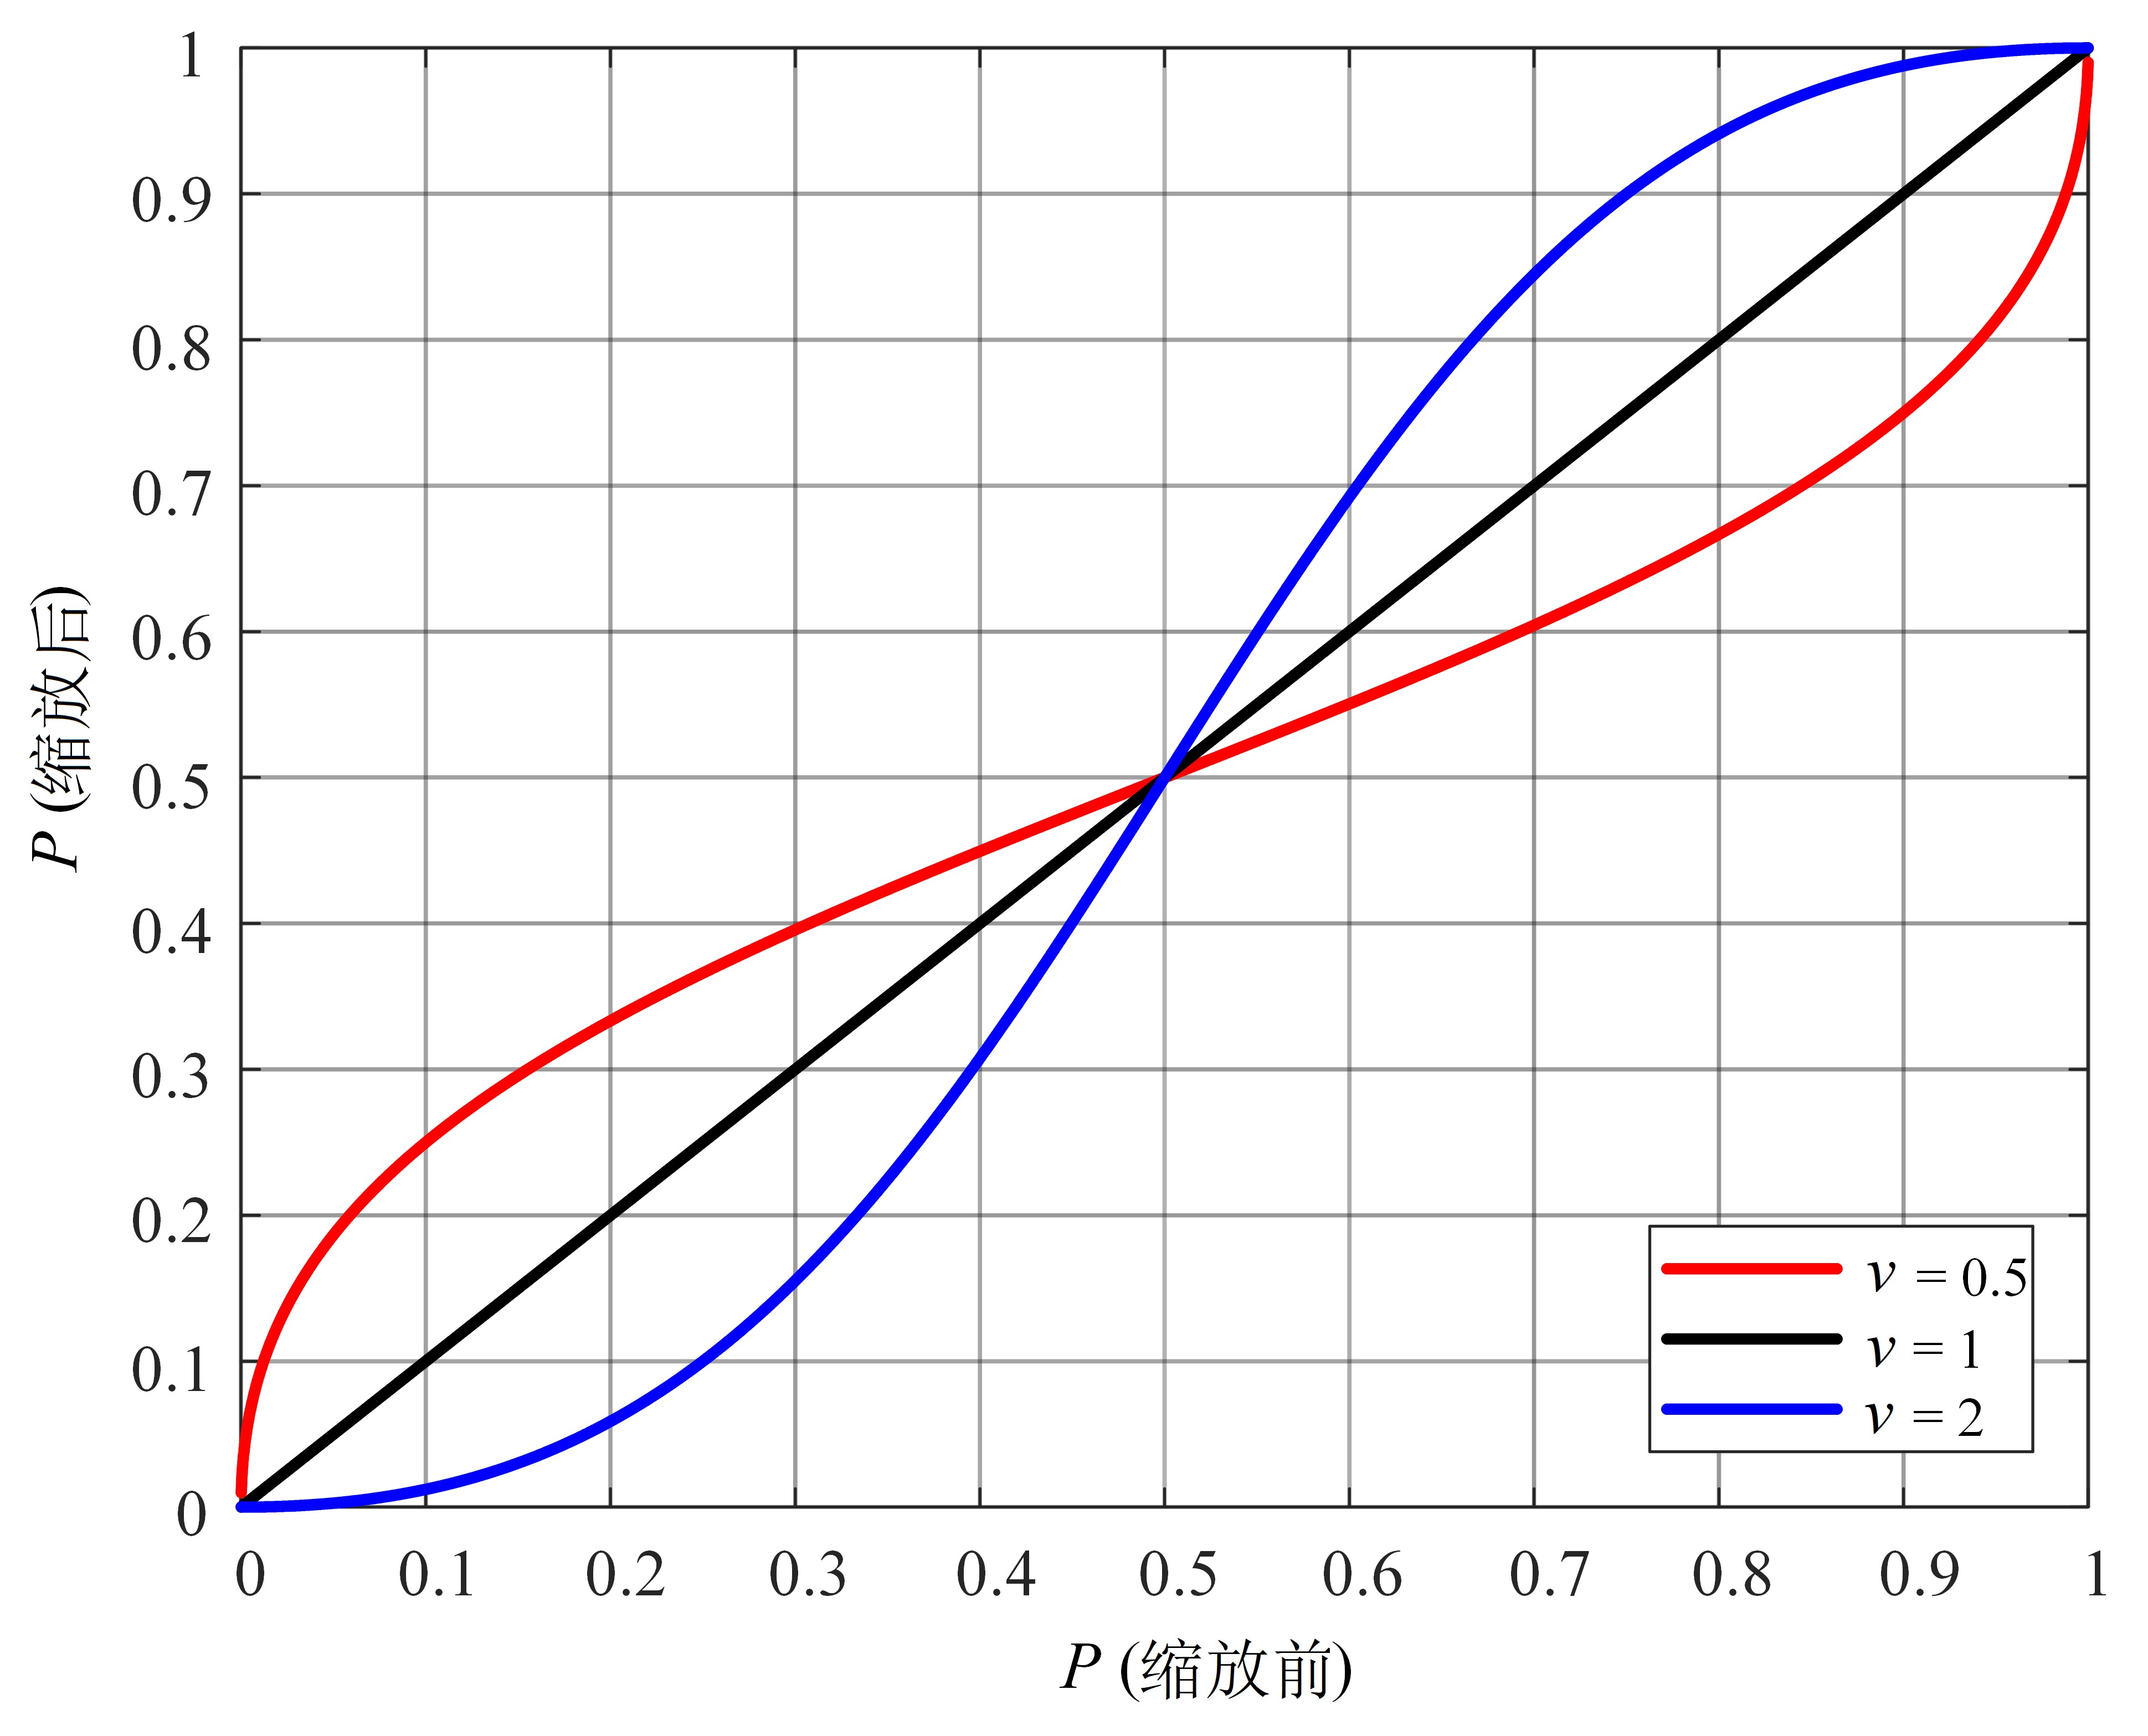
\includegraphics[width=10cm]{chapters/31}
	    \bicaption[\xiaosi 不同缩放系数v的缩放效果]{\wuhao 不同缩放系数v的缩放结果}{\wuhao Scaling results with different scaling coefficients ν}
	   	 \label{fig:3.1}
\end{figure}

%调整图片与下方文字之间的间距
\vspace{-0.35cm}

图片标题与图片之间的间距使用默认设置即可,与上下文的间距由于LATEX动态排版特性,需要大家手动调整。

。

。

。

。

。

。

。

。



下图是多子图示例:
%\vspace{-1cm}



\begin{figure}[h]
	\centering
	\subfigure[]{
		\label{fig:DE_J}
		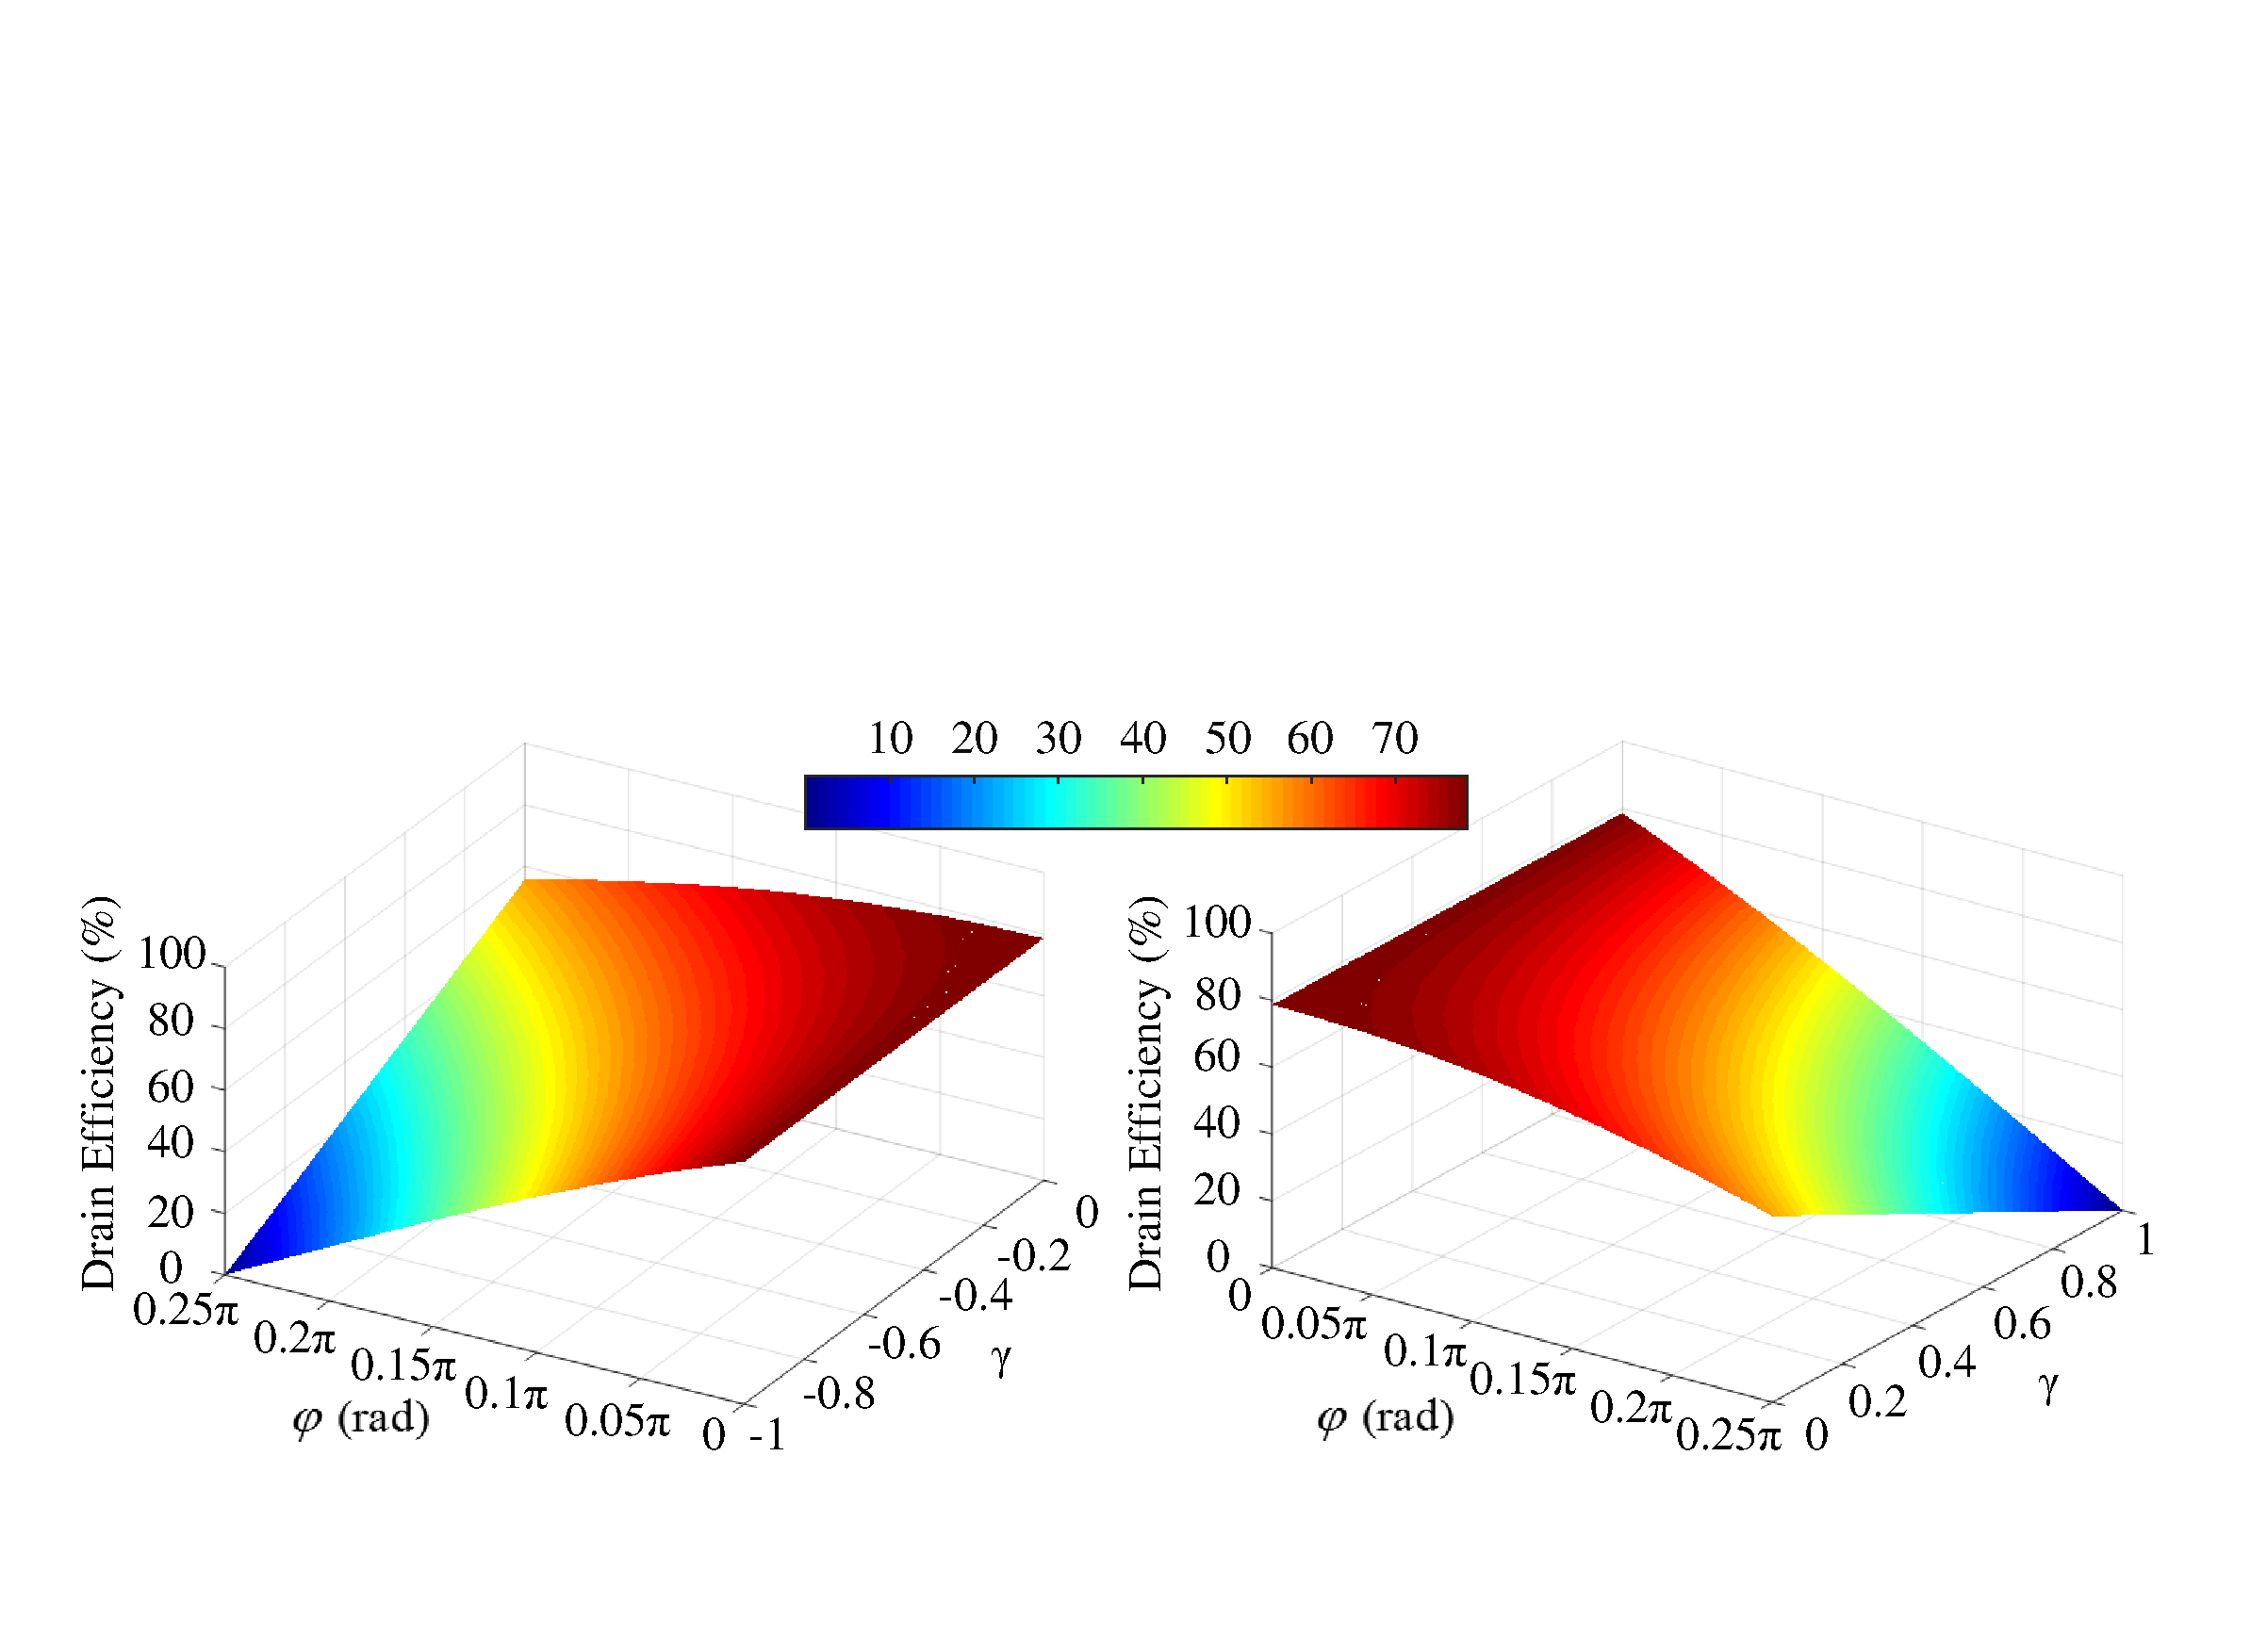
\includegraphics[width=12cm]{chapters/DE_J.pdf}}
	\subfigure[]{
		\label{fig:DE_CF}
		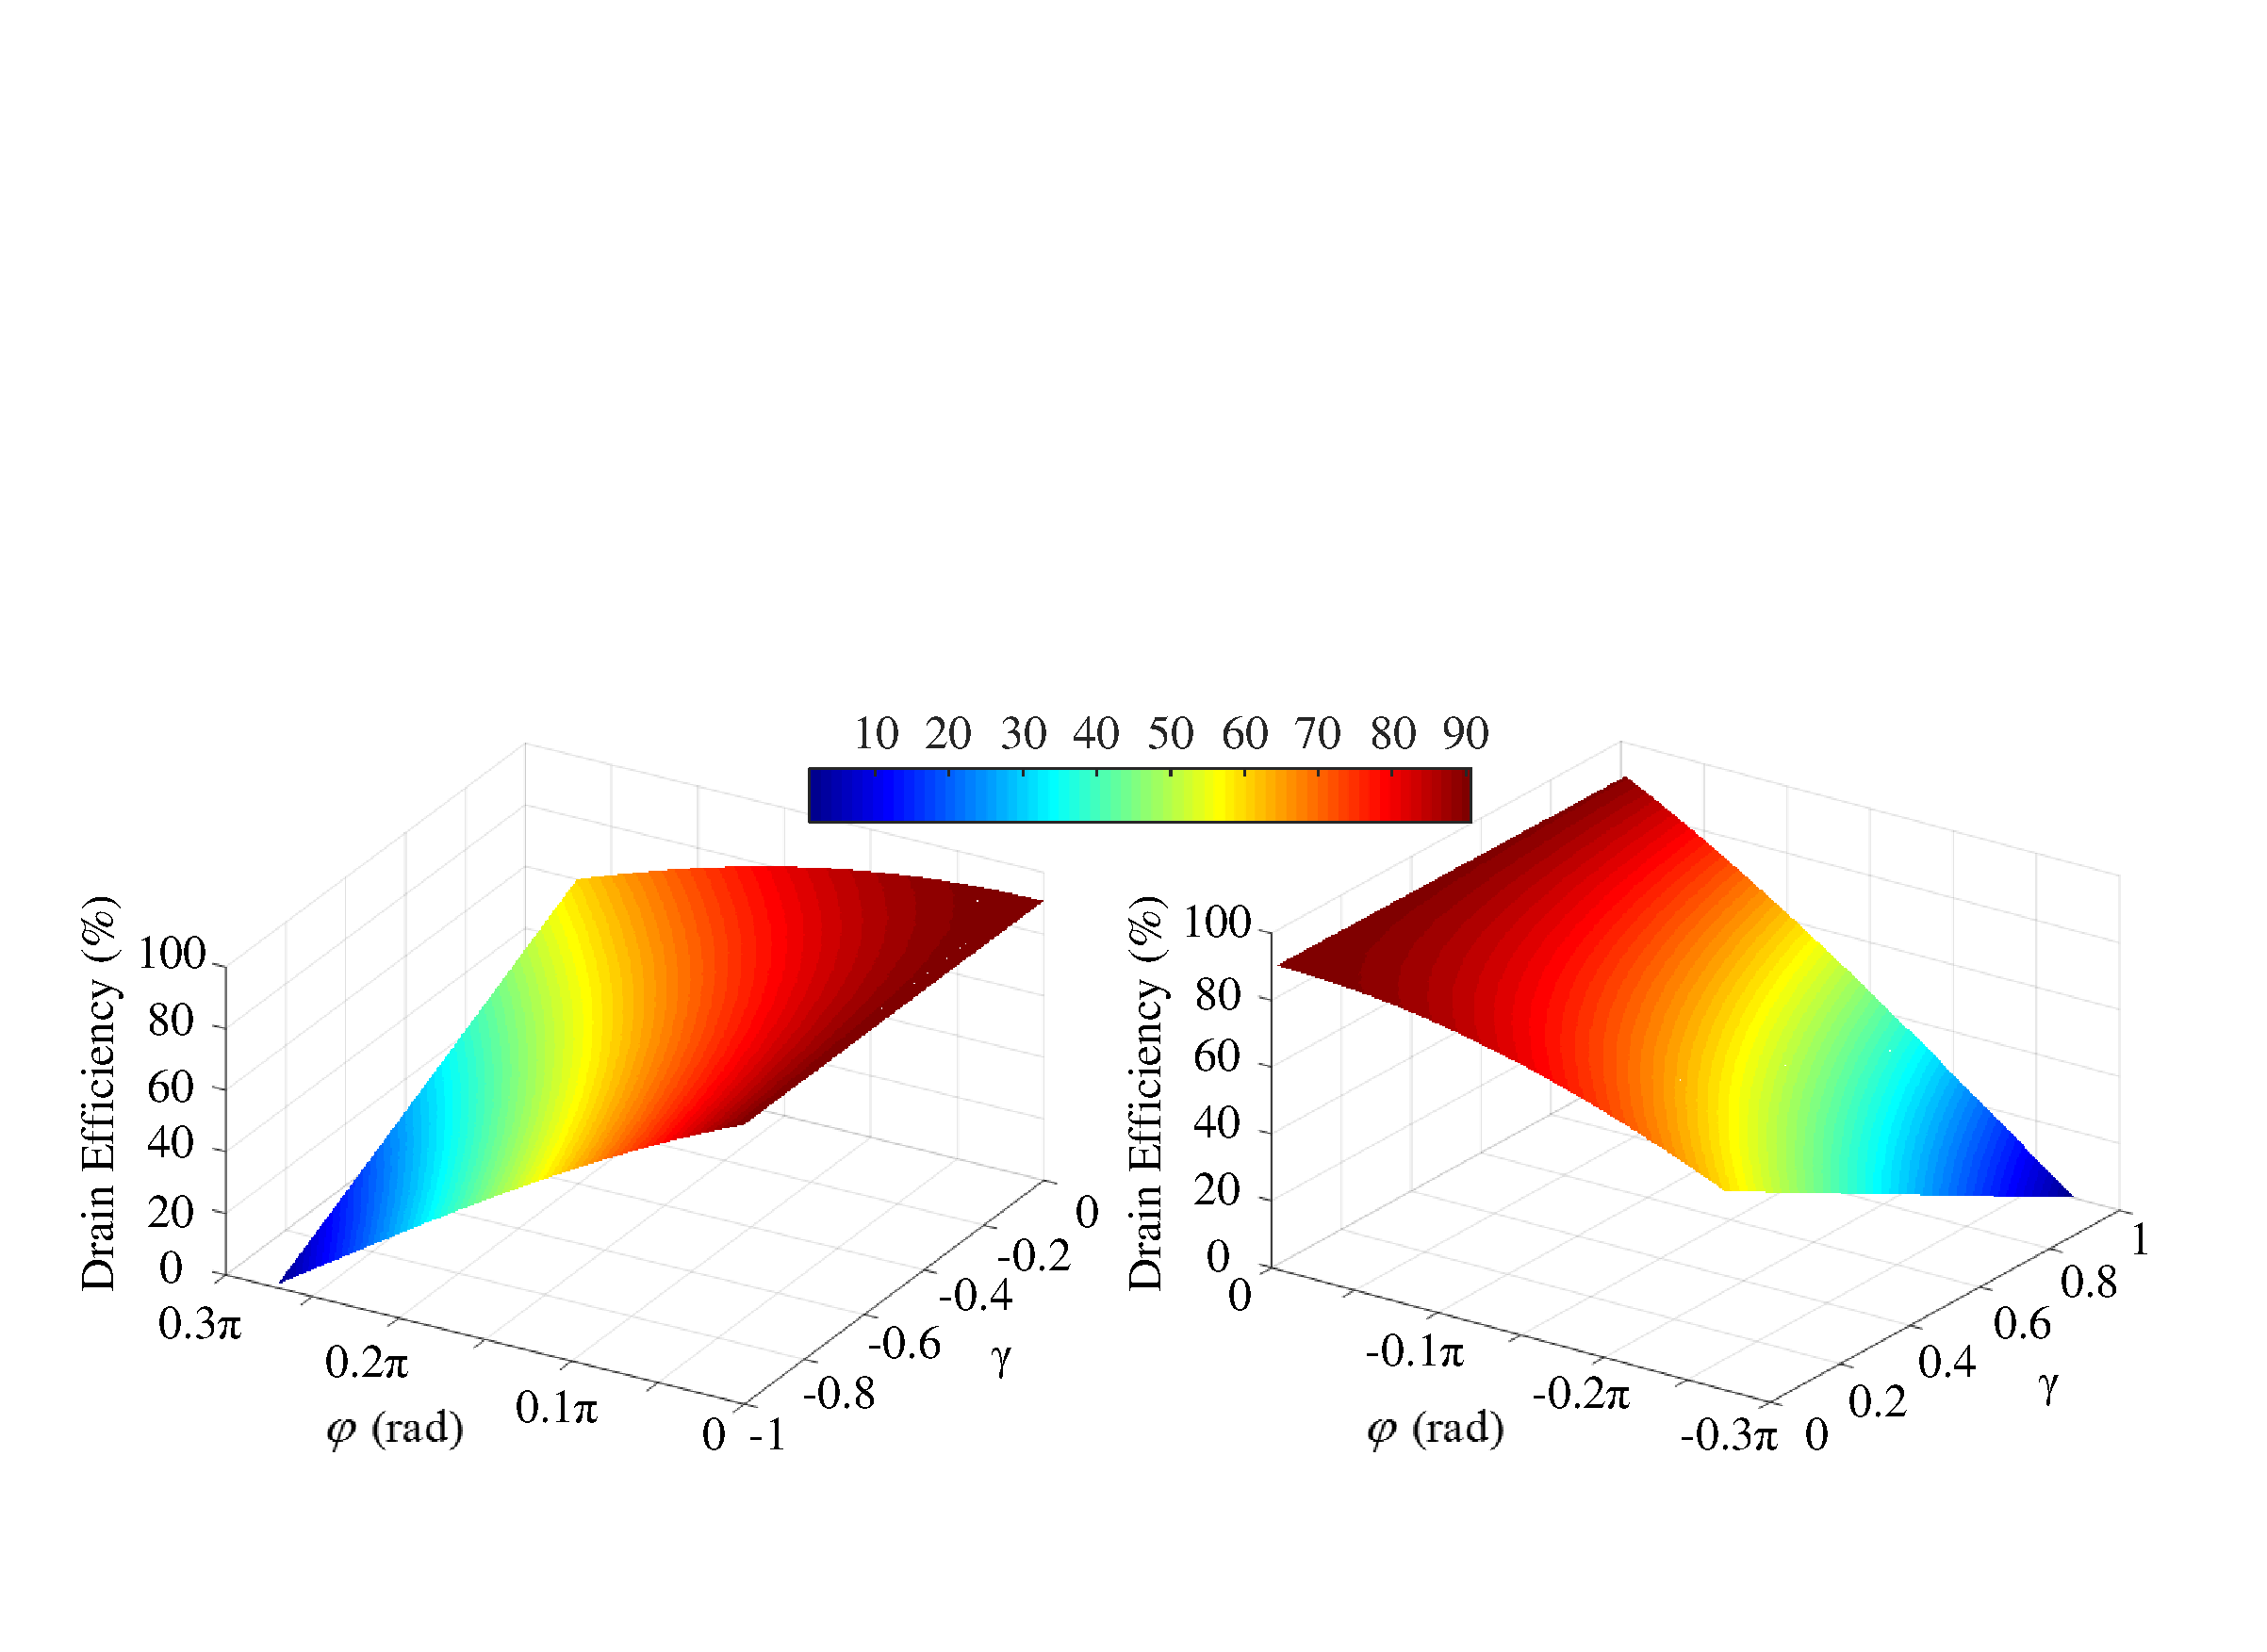
\includegraphics[width=12cm]{chapters/DE_CF.pdf}}   
\bicaption[\xiaosi 理论效率与$\gamma$和$\varphi$的关系。]{\wuhao 理论效率与$\gamma$和$\varphi$的关系。 (a) $\alpha=1$; (b) $\alpha=2/\sqrt{3}$}{\wuhao Theoretical DE versus $\gamma$ and $\varphi$. (a) $\alpha=1$; (b) $\alpha=2/\sqrt{3}$}

%	\caption{\wuhao 理论效率与$\gamma$和$\varphi$的关系。 (a) $\alpha=1$; (b) $\alpha=2/\sqrt{3}$}
%%	\raggedright
%	\wuhao Fig. 3-2 Theoretical DE versus $\gamma$ and $\varphi$. (a) $\alpha=1$. (b) $\alpha=2/\sqrt{3}$.Theoretical DE versus $\gamma$ and $\varphi$. (a) $\alpha=1$. (b) $\alpha=2/\sqrt{3}$.
\end{figure}

\vspace{-0.5cm}

\subsection{表}

表格格式参照写作指南。表格格式参照写作指南。表格格式参照写作指南。表格格式参照写作指南。表格格式参照写作指南。表格格式参照写作指南。表格格式参照写作指南。表格格式参照写作指南。表格格式参照写作指南。表格格式参照写作指南。表格格式参照写作指南。表格格式参照写作指南。表格格式参照写作指南。表格格式参照写作指南。表格格式参照写作指南。表格格式参照写作指南。

\vspace{0.1cm}

\begin{table}[h]
	\renewcommand{\arraystretch}{1.5}
	\centering
	\bicaption[\xiaosi 电流类型对效率的影响]{\wuhao 电流类型对效率的影响}{\wuhao Current type impact on efficiency}
	\begin{tabular}{p{3cm}p{3cm}p{3cm}p{3cm}}
		\toprule[1.5pt]
		\makecell[c]{\songti\wuhao 电流类型}&\makecell[c]{\songti\wuhao A}&\makecell[c]{\songti\wuhao B}&\makecell[c]{\songti\wuhao C}\\
		\hline
		\makecell[c]{\wuhao aaa}&\makecell[c]{\wuhao aa1}&\makecell[c]{\wuhao bb1}&\makecell[c]{\wuhao cc1}\\
		\bottomrule[1.5pt]
	\end{tabular}
   \label{tab:3.1} 	
\end{table}

表格格式参照写作指南。表格格式参照写作指南。表格格式参照写作指南。表格格式参照写作指南。表格格式参照写作指南。表格格式参照写作指南。表格格式参照写作指南。表格格式参照写作指南。表格格式参照写作指南。表格格式参照写作指南。表格格式参照写作指南。表格格式参照写作指南。表格格式参照写作指南。表格格式参照写作指南。表格格式参照写作指南。表格格式参照写作指南。

\vspace{-0.1cm}

\begin{table*}[h]
	\renewcommand{\arraystretch}{1.5}
	\bicaption[\xiaosi 高效率功放性能对比]{\wuhao 高效率功放性能对比}{\wuhao High-effiency power amplifier performance comparison}
	\label{tab_1}
	\centering
	\wuhao
	\begin{tabular}{c c c c c }
		\hline
		{\textbf{带宽}(GHz)}&{\textbf{功率}(dBm)}&{\textbf{效率}(\%)}&{\textbf{线性度}(dBc)}&{\textbf{信号带宽}(MHz)}\\
		\hline
		1.4--2.6&32--34&30--40 (DE)&-25 -- -30 (ACLR)&5\\
		\hline
		\multirow{2}{*}{2.1--2.7}&39&45 (DE) @ 2.14 GHz&--31 (ACLR)&\multirow{2}{*}{5}\\\cline{3-4}
		&(average)&40 (DE) @ 2.655 GHz&--30 (ACLR)&\\
		\hline
		3.5&38.1&59 (PAE)&30 (C/I)&5\\
		\hline
		\multirow{2}{*}{1.6--2.6}&36.0--38.5&45--60 (PAE)&30 (C/I)&5\\\cline{2-5}
		&35.3--37.5&40--55 (PAE)&--30 (ACLR)&20\\
		\hline
	\end{tabular}
\end{table*}


\section{公式格式}

\begin{equation}
\left\{ \begin{aligned}
0.794 \le \zeta  \le 1 ~~~~~~~~~~~\\
0.631 \le \gamma  = \frac{{0.631}}{{{\zeta ^2}}} \le 1~~~~~~ \\
- \frac{1}{{2\gamma }} \le \delta  \le \frac{1}{{2\gamma }}~~~~~~~~~~~ \\
{Z_{c,low,f}} = 2{R_{opt}}(\gamma  + j\delta )~~~~~\\
{Z_{c,2f}} = {Z_{c,low,2f}} =  - j\frac{{3\pi }}{4}\gamma \delta {R_{opt}}
\end{aligned} \right.
\label{eq:3.1}
\end{equation}

\begin{equation}
\begin{aligned}
v(\theta ) = V_{DD}\cdot(1 - \alpha cos(\theta  + \varphi ) + \beta cos(3\theta  + 3\varphi ))\\
\cdot(1 - \gamma \sin (\theta  + \varphi )) ~~~~~- 1 \le \gamma  \le 1\
\end{aligned}
\label{eq:vd}
\end{equation}




\noindent
公式格式测试。${\mathbf{\Theta }} = \left\{ {{\theta _k}\left( n \right),\forall k,n} \right\}$

\section{印制要求}
涉密学位论文的印刷、制作、传递、存档等,须符合国家、学校相关保密要求。学位论文一律左侧装订。

中文摘要之前的前置部分(封面、中、英文题名页、独创性声明和使用授权书),采用单面印刷。

从中文摘要开始,采用双面印刷。

中文摘要及之后的前置部分,包括中文摘要、ABSTRACT、目录、图目录(如有)、表目录(如有)、主要符号表(如有)、缩略词表(如有),在双面印刷时,若某部分页数为奇数,则该部分最后一页单面印刷。例如:若“摘要”只有1页,则其页码是“Ⅰ”,第“Ⅰ”页纸的背面为空白(无页眉或页码);“ABSTRACT”用新的一张纸印刷,页码从“Ⅱ”开始。

从第1章第1页开始,至论文最后1页,所有页面均双面印刷。例如:若第1章的最后1页为第17页,则第2章的第1页在第17页的背面印刷,页码为“18”(页眉是“重庆邮电大学博士(硕士)学位论文”)。

一次性双面打印整本学位论文技巧:除用于打印的版本外,电子版论文中一律不得出现空白页。论文打印建议使用PDF格式。为方便一次性双面打印,有时可在单面印刷的部分(如封面、中、英文题名页、独创性声明和使用授权书),或者双面打印只有1页的某部分内容(如摘要、ABSTRACT等)后插入1页空白页,该空白页不编排页眉页码;论文中出现的页码应前后连续,不得中断。


\section{本章小结}
本章介绍了……